\documentclass[sigconf,natbib=true,anonymous]{acmart}
%% RecSys 2026 — Main Track Long Paper (8 pages content + unlimited references)
%% Uses ACM sigconf format (two-column layout), double-blind review.
%% Camera-ready: remove 'anonymous' and add author info.

%% Remove ACM-specific elements for cleaner review copy
\settopmatter{printacmref=false}
\renewcommand\footnotetextcopyrightpermission[1]{}
\setcopyright{none}
\acmConference[RecSys'26]{Proceedings of the 20th ACM Conference on Recommender Systems}{September 2026}{TBD}
\acmYear{2026}
\acmDOI{}
\acmISBN{}

\usepackage{booktabs}
\usepackage{multirow}
\usepackage{amsmath,amssymb}
\usepackage{algorithm}
\usepackage{algpseudocode}
\usepackage{graphicx}
\usepackage{subcaption}
\usepackage{siunitx}
\usepackage{xspace}
\usepackage{enumitem}
\usepackage{microtype}
% Extra stretch in two-column mode reduces overfull lines (ACM sigconf).
\setlength{\emergencystretch}{3em}
\usepackage{ifthen}
\usepackage{balance}  % Balance columns on last page
\usepackage{hyperref} % Required for \url{} in abstract & body
\usepackage{ctex} % 中文正文（建议用 XeLaTeX 编译）

\newcommand{\model}{\textsc{MV-Align}\xspace}
\newcommand{\base}{\textsc{SASRec}\xspace}
\newcommand{\tfidf}{\textsc{TF-IDF}\xspace}
\newcommand{\llm}{\textsc{LLM}\xspace}
\newcommand{\InfoNCE}{InfoNCE\xspace}

% Circled numbers for figure captions (using textcomp to avoid tikz/amssymb conflict)
\usepackage{pifont}
\newcommand*\circled[1]{\ding{\numexpr171+#1\relax}}

% Breakable slash lists (e.g., view names) — unbreakable `/` runs often overfill columns.
\newcommand{\slashbreak}{/\allowbreak{}}

\begin{document}

\title{MV-Align：面向序列推荐的显式特征交叉多视角文本对齐}

% Review version: anonymous authors.
% Camera-ready example:
% \author{First Author}
% \affiliation{\institution{Institution}\country{Country}}
% \email{email@example.com}

\begin{abstract}
将文本特征融入序列推荐器可显著提升泛化能力，尤其对冷启动物品尤为明显；然而既有方法往往依赖单一文本表示，并仅通过共享注意力层与 ID 嵌入隐式融合。
我们认为该设计错失了两点机会：(i)~由多样化提示驱动的多视角 \llm 表征能捕捉单一嵌入无法覆盖的互补物品语义；(ii)~在点击率预测中已得到充分验证、但在序列推荐中尚少探索的 ID 与文本信号之间的\emph{显式特征交叉}，可提升排序质量。
%
我们在 \base 骨干之上提出 \model，并协调引入三项设计：融合前对多视角 \llm 嵌入去相关的\emph{逐视角白化}、通过 DCN-V2 实现的\emph{显式 ID$\times$Text 交叉交互}，以及带冷启动重加权的\emph{多视角对比对齐}。
在 Amazon Beauty 与 Toys\&Games 上采用全量排序评估与受控消融，我们实证刻画了全量排序下的\textbf{HR--排序权衡}：启用交叉网络会以召回（HR）为代价提升排序精度（MRR/NDCG），而关闭则会逆转该平衡——该结论可直接对应候选生成与最终重排在部署层面的取舍。
%
\model 取得 HR@10 为 \textbf{5.79}\% 与 \textbf{6.61}\%（相对仅 ID 分别 +6.8\% 与 +11.7\%）；在嵌入带宽相同的前提下，多视角提示在 Beauty 上将冷启动 HR\_new 与仅 ID 的差距缩小至 1.76\% 对 1.88\%，在 Toys 上则超过仅 ID（2.04\% 对 1.92\%），并在两个数据集上均取得最优的冷启动排序质量（NDCG\_new 与 MRR\_new）。
代码与配置见 \texttt{\url{https://anonymous.4open.science/r/recbole-multiview-D83A}}。
\end{abstract}

\keywords{序列推荐, 文本增强推荐, \mbox{多视角}表示, 特征交叉, 对比对齐, \mbox{冷启动}}

\maketitle

\section{引言}

诸如 \base~\cite{kang2018sasrec} 等现代序列推荐器为建模用户行为序列提供了强骨干，
但现实目录往往由冷启动与长尾物品主导，协同信号稀疏。物品文本（标题、描述、评论等）
可提供有助于泛化的语义线索，却也带来工程上的张力：轻量特征（如 \tfidf）成本低且
 出人意料地强，而 \llm 嵌入往往更丰富，但在抽取、存储与在线服务上代价高得多。

一个自然的问题是：多视角 \llm 特征是否值得额外复杂度。我们通过报告可训练参数量与
前向 FLOPs（表~\ref{tab:params}），并在 \S\ref{sec:complexity} 分析离线编码成本来量化。

两点实践观察驱动本文。首先，在已有较强 \tfidf 基线时（例如 Beauty 全量排序下
HR@10 +2.6\%、NDCG@10 +25.9\%），再叠加 \llm 的边际增益可能较小且领域相关，
何时值得为多视角提示付出额外离线编码与适度可训练开销并不明朗（\S\ref{sec:experiments}）。
其次，工业界模型选型常依赖快速采样评估（如 uniform-100 负例），但采样指标可能与
全量排序指标不一致甚至错排模型~\cite{krichene2020sampledmetrics}；当改进集中在
冷启动/长尾层时，这种错配尤其有害。

\model 以简单的 ``prepare--interact--align'' 流程化解上述矛盾（图~\ref{fig:framework}）：

\textbf{(1) Prepare}（表征层）：我们对各文本视角独立归一化与白化，以应对三类失效模式——
跨视角尺度不匹配、视角间相关性与跨视角冗余。白化使多视角通道去相关，后续交互更易学习。

\textbf{(2) Interact}（融合层）：我们使用显式交叉网络（DCN-V2）学习高阶 ID$\times$text 特征交叉。
Transformer 自注意力虽建模序列级物品--物品依赖，却不显式刻画 ID 与文本嵌入之间的特征级交互；
DCN-V2 通过由可学习权重矩阵门控的逐元素乘积填补该缺口。

\textbf{(3) Align}（目标层）：我们通过 InfoNCE 对比损失将各文本视角对齐到协同 ID 嵌入空间。
对齐方向为（文本视角 $\to$ ID 空间）；正样本为（物品文本视角，物品 ID 嵌入）；负样本为批内物品。
\mbox{冷启动}重加权避免高频物品主导对齐信号，使低流行度物品获得足够梯度更新。

我们的贡献有三点。
\begin{itemize}[leftmargin=*,itemsep=1pt]
  \item \textbf{系统方法设计。} 提出 \model，将显式交叉网络（DCN-V2）与多视角 \llm 文本特征
    结合用于序列推荐。``prepare--interact--align'' 联合利用逐视角白化、显式 ID$\times$Text 交叉
    与带冷启动重加权的对比对齐——据我们所知，该组合在此设定下尚未被探索。
  \item \textbf{新的实证发现。} 在两个 Amazon 领域上全量排序评估与受控消融，并结合 popularity 分层，
    揭示此前未报告的\textbf{HR--排序权衡}：交叉网络以召回（HR）为代价提升排序质量（MRR/NDCG），
    为候选生成与最终重排配置之间的工程取舍提供可操作建议。
  \item \textbf{实践设计洞见。} 轻量 \tfidf 单独已是强基线；在嵌入带宽相同（$4{\times}64$-d 对
    $1{\times}256$-d）时，多视角提示稳定优于单视角，冷启动物品上增益最大。
\end{itemize}
围绕四个研究问题组织：\textbf{RQ1}~逐视角白化是否提升文本特征质量？
\textbf{RQ2}~SE 式通道门控是否有帮助？
\textbf{RQ3}~带宽相同时多视角是否优于单视角？
\textbf{RQ4}~显式交叉与对比对齐各自贡献如何？
本文结构：相关工作、\model 方法、全量排序结果与消融，最后为分析与结论。

%% [Figure 1 (cover/teaser) removed per advisor feedback — overlaps with Figure 2.
%%  Retained in anonymous repository for poster / presentation use.]

\section{相关工作}
\paragraph{序列推荐。}
基于 Transformer 的序列模型如 \base~\cite{kang2018sasrec} 与 BERT4Rec~\cite{sun2019bert4rec}
（双向掩码预测）是刻画用户行为模式的强骨干。GRU4Rec~\cite{hidasi2016gru4rec} 开创 RNN 会话建模，
SASRec 则以因果掩码的自注意力做下一物品预测。近期高效变体包括以低秩注意力分解降低复杂度的
LightSANs~\cite{fan2021lightsans}。

\paragraph{文本增强推荐。}
\begin{sloppypar}
物品文本特征（词袋、神经编码器或 \llm 嵌入）在协同过滤之外提供互补信号。早期工作用 TF-IDF 与
Item2Vec~\cite{barkan2016item2vec} 表示物品；CDL~\cite{wang2015cdl} 通过堆叠去噪自编码器联合建模文本。
近期方法利用预训练语言模型：UniSRec~\cite{hou2022unisrec} 将 BERT 编码的文本作为可迁移表示，
VQ-Rec~\cite{hou2023vqrec} 通过向量量化桥接语言与协同语义。大语言模型进一步拓展该方向：
P5~\cite{geng2022p5} 以 text-to-text 范式统一推荐，TALLRec~\cite{bao2023tallrec} 通过指令微调对齐 LLM 与推荐。
然而这些方法通常以单一提示或表征编码物品文本。本文探索通过多样提示视角（身份、功能、受众、品类等）
的\emph{多视角} \llm 嵌入，并结合显式融合与对齐，说明相对更简单基线何时值得引入该复杂度。
\end{sloppypar}

\paragraph{特征交互与交叉网络。}
\begin{sloppypar}
Deep \& Cross Network (DCN)~\cite{wang2017dcn} 及其后继 DCN-V2~\cite{wang2021dcnv2} 显式建模特征交叉，
与 DNN 学到的隐式交互互补。Squeeze-and-Excitation (SENet)~\cite{hu2018senet} 引入通道注意力做特征重标定；
FiBiNET~\cite{huang2019fibinet} 将 SENet 适配到 CTR 并结合双线性特征交互。推荐中交叉网络在 CTR 上已见成效；
本文将其用于序列设定下的 ID--文本融合，并以 SE 式模块对 \llm 特征做逐视角通道门控。
\end{sloppypar}

\paragraph{推荐中的多视角学习。}
多视角学习利用不同特征源或模态的互补信息。受 CLIP~\cite{radford2021clip} 通过对比学习对齐视觉与文本启发，
我们设计多视角提示从语言模型中引出多样语义。推荐中会话场景已有图神经网络多视角探索~\cite{huang2025mvcgnn_session}。
本文将多视角学习用于 \llm 文本嵌入，采用不同提示视角（身份、功能、受众、品类）并在融合前白化以去相关。

\paragraph{推荐中的对比学习。}
\InfoNCE~\cite{oord2018cpc} 等对比目标广泛用于自监督表征学习。推荐中对比方法对齐跨视角的用户/物品表示~\cite{wu2021cl4rec}。
本文将其扩展为带冷启动重加权的多视角 text-to-ID 对齐。

\paragraph{评估协议。}
采样评估可能误导模型选择~\cite{krichene2020sampledmetrics}；全量排序更可靠但计算昂贵。本文采用全量排序与分层分析，
以理解不同 popularity 层上的行为。

%% [RecSys] Research Questions section removed — RQs folded into Introduction above.

\section{方法}
图~\ref{fig:framework} 展示 \model 的整体架构，包含三个关键部分：
(1)~\textbf{归一化与白化}，各文本视角逐视角归一化以缓解各向异性；
(2)~\textbf{交叉网络}，通过 DCN-V2 捕获显式 ID$\times$Text 交互；
(3)~\textbf{多视角对齐}，以带冷启动重加权的 InfoNCE 将文本视角与 ID 嵌入对齐。
下文分述各模块。

\subsection{骨干：带文本融合的 SASRec}
设用户交互序列为 $s_u = [i_1,\dots,i_n]$，最大长度 $L$。\base 通过 Transformer 将 $s_u$ 编码为
序列表示 $\mathbf{h}_u \in \mathbb{R}^d$。每个物品 $i$ 有 ID 嵌入 $\mathbf{e}_i \in \mathbb{R}^d$。
我们用文本特征增强物品并将其融合为用于打分的\emph{融合物品嵌入} $\tilde{\mathbf{e}}_i$。

\subsection{多视角文本表示}\label{sec:whiten}
假设轻量 \tfidf 嵌入 $\mathbf{t}_i^{(0)} \in \mathbb{R}^{d_t}$ 为基视角，另有 $V$ 个 \llm 提示视角
$\{\mathbf{t}_i^{(v)} \in \mathbb{R}^{d_l}\}_{v=1}^V$（例如身份\slashbreak{}功能\slashbreak{}受众\slashbreak{}品类），
$d_t$、$d_l$ 分别为 \tfidf 与原始 \llm 嵌入维度。

\paragraph{逐视角白化。}
多视角 \llm 嵌入存在三类失效模式：\textbf{(i) 尺度不匹配}——不同视角幅度分布差异大，部分视角主导融合；
\textbf{(ii) 视角相关}——语义相近的提示产生相关特征，冗余编码相同信息；\textbf{(iii) 跨视角冗余}——
未去相关时交叉网络易学到跨视角冗余交互而非互补交叉。

为此先将各 \llm 视角由 $d_l$ 截断 SVD 降至 $d_v$ 维，再对各视角独立施加 ZCA 白化~\cite{kessy2018zca}，
使多视角通道去相关、后续交互更易学习。给定全体物品在视角 $v$ 上的降维矩阵 $\mathbf{X}^{(v)} \in \mathbb{R}^{|I| \times d_v}$，
计算：
\begin{align}
  \mathbf{X}_c^{(v)} &= \mathbf{X}^{(v)} - \boldsymbol{\mu}^{(v)}, \\
  \boldsymbol{\Sigma}^{(v)} &= \frac{1}{|I|}(\mathbf{X}_c^{(v)})^\top \mathbf{X}_c^{(v)}, \\
  \mathbf{X}_w^{(v)} &= \mathbf{X}_c^{(v)} (\boldsymbol{\Sigma}^{(v)} + \epsilon \mathbf{I})^{-1/2},
\end{align}
其中 $\boldsymbol{\mu}^{(v)}$ 为均值嵌入，$\boldsymbol{\Sigma}^{(v)}$ 为协方差矩阵，
$\epsilon$ 为小常数以保证数值稳定。白化统计在训练集上离线计算，训练\slashbreak{}推理阶段固定。
各视角使用独立白化参数（逐视角白化），较跨视角共享白化更能保留视角特有语义。

\paragraph{SE 式通道门控。}
我们采用 SE 式通道门控做自适应特征重标定，灵感来自 SENet~\cite{hu2018senet} 的通道注意力。
原版 SENet 先 squeeze（全局池化）再 excitation；本文对每个投影后的嵌入直接做 MLP 门控，
更适合逐物品表示（跨物品不做池化）。各白化视角先投影到骨干维度 $d$，再按下式精炼：
\begin{align}
  \mathbf{z}_i^{(v)} &= \mathbf{W}_v \mathbf{t}_{w,i}^{(v)} \in \mathbb{R}^d,\\
  \mathbf{r}_i^{(v)} &= \mathbf{z}_i^{(v)} \odot \sigma(\mathrm{MLP}_v(\mathbf{z}_i^{(v)})),
\end{align}
其中 $\mathbf{W}_v \in \mathbb{R}^{d \times d_v}$ 为投影矩阵，
$\mathbf{t}_{w,i}^{(v)} \in \mathbb{R}^{d_v}$ 为物品 $i$ 在视角 $v$ 的白化嵌入，
$\mathrm{MLP}_v: \mathbb{R}^d \to \mathbb{R}^d$ 为两层网络，压缩比 $r$。

\paragraph{逐视角 $\ell_2$ 归一化。}
SE 式门控后，我们对各视角独立做 $\ell_2$ 归一化，目的有二：
(i) 使各视角以可比尺度参与融合，避免幅度大的视角主导；(ii) 为后续交叉网络提供良态输入以稳定学习：
\begin{equation}
  \hat{\mathbf{r}}_i^{(v)} = \frac{\mathbf{r}_i^{(v)}}{\lVert \mathbf{r}_i^{(v)} \rVert_2 + \epsilon}.
\end{equation}
与白化配合，逐视角归一化在保留各视角语义的同时缓解跨视角尺度不匹配：白化去相关各视角内部维度，
$\ell_2$ 归一化使跨视角贡献幅度可比。

\paragraph{视角门控与融合。}
为每个视角学习标量门 $g_v=\sigma(\theta_v)\in(0,1)$，且\emph{不}强制跨视角归一化（各视角独立贡献 $0$--$1$）。
所有视角（及可选的 \tfidf 基）拼接后投影回 $\mathbb{R}^d$：
\begin{equation}
  \mathbf{t}_i = \mathbf{P}\Big[\mathbf{t}_i^{(0)};\; g_1\hat{\mathbf{r}}_i^{(1)};\; \dots;\; g_V\hat{\mathbf{r}}_i^{(V)}\Big] \in \mathbb{R}^d,
\end{equation}
其中 $\mathbf{P} \in \mathbb{R}^{d \times (d_t + Vd)}$ 为融合投影矩阵。

\subsection{显式交叉融合}\label{sec:cross}
除依赖自注意力捕获协同与文本信号的高阶交互外，我们引入基于 DCN-V2~\cite{wang2021dcnv2} 的\emph{显式交叉}模块。
\base 中的自注意力建模序列级物品--物品依赖，但不显式刻画 ID 与文本嵌入之间的特征级交叉；DCN-V2 通过
可学习权重矩阵门控的逐元素乘积学习高阶 ID$\times$text 交互。

给定拼接特征 $\mathbf{x}_i=[\mathbf{e}_i;\alpha_i \mathbf{t}_i] \in \mathbb{R}^{2d}$，其中 $\mathbf{e}_i \in \mathbb{R}^d$ 为 ID 嵌入，
$\mathbf{t}_i \in \mathbb{R}^d$ 为融合后的文本表示，交叉层更新为：
\begin{equation}
  \mathbf{x}^{(l+1)} = \mathbf{x}^{(l)} + \mathbf{x}^{(0)} \odot (\mathbf{W}_l\mathbf{x}^{(l)} + \mathbf{b}_l),
\end{equation}
其中 $\mathbf{W}_l \in \mathbb{R}^{2d \times 2d}$ 为满秩权重矩阵，$\mathbf{b}_l \in \mathbb{R}^{2d}$ 为偏置；
$\odot$ 表示逐元素乘积。我们采用 DCN-V2 的满秩（非 mix）变体，而非低秩或混合专家变体。
交叉输出 $\mathbf{x}^{(C)} \in \mathbb{R}^{2d}$ 与浅层 MLP 经预测层组合得到融合嵌入 $\tilde{\mathbf{e}}_i \in \mathbb{R}^d$。
标量 $\alpha_i \in (0,1)$ 包含全局文本门控与可选的逐物品门控，并辅以温度缩放以稳定融合。

\subsection{多视角对比对齐}\label{sec:align}
我们使用 \InfoNCE~\cite{oord2018cpc} 将各文本视角对齐到 ID 嵌入空间。对齐方向为\textbf{文本视角 $\to$ ID 空间}；
正样本为（物品文本视角，物品 ID 嵌入）；负样本为批内物品。这样文本表示携带协同信号，可在冷启动场景下
作为 ID 嵌入的即插即用替代。

对批量大小为 $B$ 的物品，定义余弦相似度矩阵 $\mathbf{S} \in \mathbb{R}^{B \times B}$，元素为
$\mathbf{S}_{ij} = \mathrm{cos}(\mathbf{e}_{i},\hat{\mathbf{r}}_{j}^{(v)})$（ID 嵌入 $\mathbf{e}_i \in \mathbb{R}^d$
与文本视角嵌入 $\hat{\mathbf{r}}_j^{(v)} \in \mathbb{R}^d$），温度 $\tau$。逐视角对齐损失为：
\begin{equation}
  \mathcal{L}_{\text{align}}^{(v)} =
  \frac{1}{B}\sum_{i=1}^{B}
  -\log \frac{\exp(\mathbf{S}_{ii}/\tau)}{\sum_{j=1}^{B}\exp(\mathbf{S}_{ij}/\tau)}.
\end{equation}
We learn view weights $\pi_v=\mathrm{softmax}(\boldsymbol{\phi})_v$
and combine per-view losses:
\begin{equation}
  \mathcal{L}_{\text{mv-align}} = \sum_{v=1}^{V}\pi_v \mathcal{L}_{\text{align,w}}^{(v)}.
\end{equation}

We enhance cold-start item performance through two complementary
mechanisms that operate at different stages:

\paragraph{Training-time cold-start reweighting.}
To avoid alignment being dominated by frequent items, we
reweight samples based on item popularity $\mathrm{pop}(i)$
during training, where $\mathrm{pop}(i)$ is the interaction count:
\begin{equation}
  w_i = 1 + \beta\cdot \max\Big(0, \frac{P_0-\mathrm{pop}(i)}{P_0}\Big),
  \label{eq:cold_reweight}
\end{equation}
where $\beta>0$ controls the strength of popularity-based reweighting,
$P_0$ is the cold-start threshold (items with $\mathrm{pop}(i) < P_0$
receive boosted weights). The weighted alignment loss becomes:
\begin{equation}
  \mathcal{L}_{\text{align,w}}^{(v)} =
  \frac{1}{\sum_i w_i}\sum_{i=1}^{B} w_i \cdot
  \left[-\log \frac{\exp(\mathbf{S}_{ii}/\tau)}{\sum_{j=1}^{B}\exp(\mathbf{S}_{ij}/\tau)}\right],
\end{equation}
where $w_i$ only reweights the anchor (positive) samples, ensuring
that cold-start items receive sufficient gradient updates during
alignment training.

\paragraph{Inference-time cold-start boosting.}
To complement training-time reweighting, we apply adaptive text
weighting during inference. For an item $i$ with popularity
$\mathrm{pop}(i)$, we compute a dynamic boost factor:
\begin{equation}
  \gamma_i = 1 + \beta_{\text{infer}} \cdot \max\Big(0, 
  \frac{P_0-\mathrm{pop}(i)}{P_0}\Big),
  \label{eq:infer_boost}
\end{equation}
where $\beta_{\text{infer}}$ is the inference boost coefficient.
The effective text weight in the fusion layer becomes 
$\alpha_i' = \alpha_i \cdot \gamma_i$, dynamically increasing text
reliance for cold-start items without modifying model parameters.
This decoupling allows deployment-time adjustment without
retraining: smaller $\beta_{\text{infer}}$ yields more balanced
overall metrics, while larger values emphasize cold-start items.
In our runs we tune $\beta_{\text{infer}}$ on validation together
with $(\lambda,\tau)$ and the training reweighting coefficient $\beta$
(Eq.~\eqref{eq:cold_reweight}); the defaults used in
\S\ref{sec:analysis} ($\beta{=}3.0$, $\beta_{\text{infer}}{=}0.6$)
reflect this trade-off.

Together, these two mechanisms ensure that cold-start items receive
both strong learning signals during training (via reweighted
alignment) and appropriate inference-time emphasis (via dynamic
boosting), enabling effective cold-start recommendations without
sacrificing performance on frequent items.

\begin{figure}[t]
\centering
\IfFileExists{figures/framework.pdf}{%
  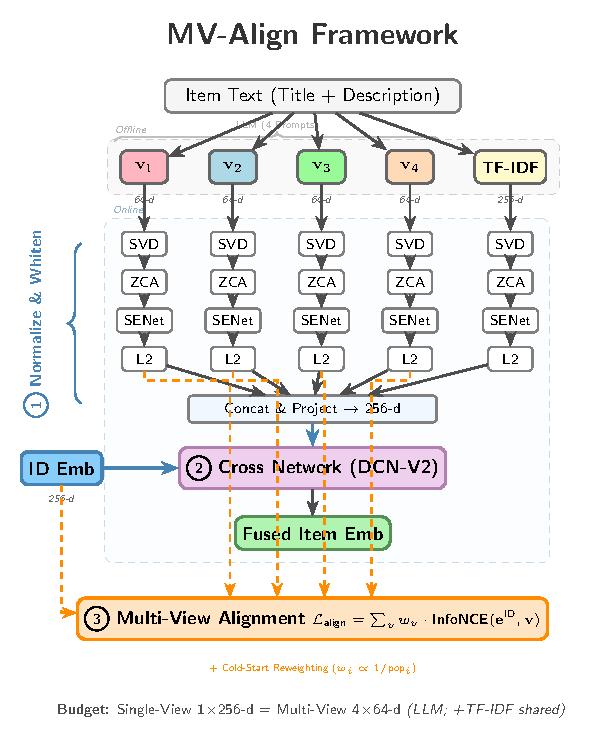
\includegraphics[width=\linewidth]{figures/framework.pdf}%
}{%
  \fbox{\parbox[c][0.22\textheight][c]{0.95\linewidth}{\centering
  \textbf{Framework figure placeholder.}\\
  Put `framework.pdf` under `paper_sigir/figures/`.}}%
}
\caption{Overview of \model.
\circled{1}~\textbf{Prepare}: per-view normalization and whitening (\S\ref{sec:whiten});
\circled{2}~\textbf{Interact}: explicit ID$\times$Text cross via DCN-V2 (\S\ref{sec:cross});
\circled{3}~\textbf{Align}: multi-view contrastive alignment with cold-start reweighting (\S\ref{sec:align}).}
\label{fig:framework}
\end{figure}

\subsection{Training Objective}
We optimize:
\begin{equation}
  \mathcal{L} = \mathcal{L}_{\text{rec}} + \lambda \cdot \mathcal{L}_{\text{mv-align}},
\end{equation}
where $\mathcal{L}_{\text{rec}}$ is the standard sequential
recommendation loss (cross-entropy with sampled negatives), and
$\lambda$ is the alignment weight. Negative sampling is used only
for training efficiency; all evaluation metrics are computed under
full ranking over the entire item set.

\subsection{Model Complexity}\label{sec:complexity}
\textbf{Offline.} \tfidf and \llm item embeddings are precomputed once
and stored as static buffers; SVD reduction and ZCA whitening are computed
offline on the training set.
Each \llm view requires a separate encoder forward pass per item, so
offline encoding cost scales roughly with the number of views (e.g.,
four prompt views vs.\ one for single-view); this is a one-time
(or periodic refresh) cost, amortized over training and serving, and
does not add per-request latency.
\textbf{Online.} The live path adds per-view projections, one DCN-V2
cross layer ($2d{\times}2d$), and fusion MLPs.
Table~\ref{tab:params} reports trainable parameters and framework-estimated
single-forward FLOPs on Amazon Beauty: text fusion and multi-view heads
add modest trainable overhead (${\sim}1.8$M parameters vs.\ \base) while
most parameters remain in the backbone and item embeddings; forward FLOPs
increase by only ${\sim}3\%$ from ID-only to multi-view.
The majority of parameters (${\sim}66$M) reside in the item embedding
table ($|I|{\times}d$); the remaining ${\sim}1$--$3$M cover Transformer
layers, text projections, and cross modules.

\subsection{Two-Phase Training Protocol}
Joint end-to-end training from scratch risks the text heads
overfitting before the backbone converges, because the randomly
initialized projections receive much larger gradients than the
pre-existing ID embeddings. We therefore adopt a two-phase schedule:
\textbf{Phase-A} (warmup) freezes the backbone and trains
text heads and cross modules with a higher learning rate,
grid-searching $(\lambda,\tau)$ on validation;
\textbf{Phase-B} (joint finetune) unfreezes all parameters
with grouped learning rates.
Both modalities are initialized together from epoch~0 so that
text heads receive learning signals while ID embeddings remain
adaptable to text-augmented representations.
Full schedule details are given in \S\ref{sec:experiments}.

\section{Experiments}\label{sec:experiments}
\subsection{Datasets and Evaluation}
We evaluate on two Amazon product review domains~\cite{mcauley2015amazon,ni2019amazon}: \textbf{Beauty} and
\textbf{Toys\&Games}. We follow time-ordered splits and
report metrics under \textbf{full ranking} at $K{=}10$.
In addition to overall metrics (HR, NDCG, MRR, Precision),
we report \textbf{popularity-stratified} metrics by item
interaction counts:
\begin{itemize}[leftmargin=*,itemsep=1pt]
  \item \textbf{new}: $[1,3)$ interactions
  \item \textbf{few}: $[3,10)$ interactions
  \item \textbf{frequent}: $[10,\infty)$ interactions
\end{itemize}
Table~\ref{tab:dataset} summarizes the dataset statistics.
We compute popularity strata from item interaction counts in
the training data.

\begin{table}[h]
\caption{Dataset statistics after 5-core filtering.}
\label{tab:dataset}
\centering
\small
\begin{tabular}{lrrrc}
\toprule
\textbf{Dataset} & \textbf{\#Users} & \textbf{\#Items} & \textbf{\#Inter.} & \textbf{Density} \\
\midrule
Beauty      & 1,210,272 & 259,217 & 2,023,071 & 0.0006\% \\
Toys\&Games & 1,342,912 & 336,080 & 2,252,772 & 0.0005\% \\
\bottomrule
\end{tabular}
\end{table}

\textbf{Main tables} (Table~\ref{tab:main}) report overall metrics and the
\textbf{new} stratum, which is most informative for cold-start;
\textbf{few} and \textbf{frequent} subtables are omitted for brevity
and included in the anonymous repository.
We report only full-ranking metrics in the
main paper, following prior findings that sampled evaluation
can mis-rank recommender models~\cite{krichene2020sampledmetrics}. Our evaluation
follows leave-one-out next-item prediction with a single
ground-truth item per test case, under which HR@K, Hit@K, and
Recall@K coincide; we use HR@K for brevity and rely on
MRR/NDCG to capture top-position quality.

\subsection{Baselines}
Our comparison design deliberately isolates the contribution of each
text-feature component under a shared backbone (\base), so that
observed gains are attributable to the text augmentation pipeline
rather than confounded by architectural differences across models.
We compare four progressively enriched configurations:
\begin{itemize}[leftmargin=*,itemsep=2pt]
  \item \textbf{\base (ID-only).} Pure sequential baseline
    without text\slashbreak{}cross\slashbreak{}align.
  \item \textbf{\base + \tfidf.} A lightweight text baseline
    using precomputed \tfidf embeddings with explicit cross
    and alignment.
  \item \textbf{\base + \tfidf + \llm (single-view).} Adds a
    single \llm embedding (Qwen2.5-7B~\cite{qwen2024qwen25}) concatenated with
    \tfidf, using SE-style gating and alignment.
  \item \textbf{\model (multi-view).} \tfidf base view + 4
    multi-view \llm prompt embeddings
    (identity\slashbreak{}function\slashbreak{}audience\slashbreak{}category) with per-view SE-style blocks,
    explicit cross, and multi-view contrastive alignment.
\end{itemize}
\noindent This layered design answers a specific question that
cross-architecture comparisons cannot: \emph{when is each additional
text component worth its cost?}
All text-enhanced variants share the same fusion/training scaffold
whenever applicable, so the comparison isolates representation choice
rather than backbone differences.
The ablation study
(\S\ref{sec:analysis}) further removes individual modules
(whitening, SE, cross, alignment) to quantify their marginal effects.

\subsection{Implementation Details}
Unless stated otherwise, we use embedding size $d=256$, max
sequence length $L=50$, 2 Transformer layers with 2 heads,
batch size 512, and Adam with base learning rate $10^{-4}$.
\paragraph{Two-phase schedule.}
We follow Phase-A ($15$ epochs) $\rightarrow$ Phase-B ($50$
epochs) with Phase-A selecting $(\lambda,\tau)$ on
$\mathrm{MRR@10}$ for both Beauty and Toys\&Games.
We use grouped learning rates:
$\text{lr}_{\text{text}}=\num{1e-3}$ for text heads,
$\text{lr}_{\text{cross}}=\num{5e-4}$ for cross/DNN blocks,
and $\text{lr}_{\text{backbone}}=\text{lr}_{\text{text}}\times
0.1$ in Phase-B.
\paragraph{Grid.}
For the main runs, we use the Balanced (default) configuration:
$\lambda=0.10$, $\tau=0.05$, training reweighting coefficient
$\beta=3.0$ (Eq.~\eqref{eq:cold_reweight}), and inference boost
$\beta_{\text{infer}}=0.6$ (Eq.~\eqref{eq:infer_boost}) on both datasets
(sensitivity in \S\ref{sec:analysis}).
\paragraph{Training and evaluation protocol.}
We run each configuration with 4 random seeds
$\{42, 2024, 2025, 2026\}$ and report mean$\pm$std;
full-ranking metrics are evaluated at $K{=}10$
with popularity stratification thresholds
\textbf{new}: $[1,3)$, \textbf{few}: $[3,10)$,
\textbf{frequent}: $[10,\infty)$. Our implementation is based on
RecBole~\cite{zhao2021recbole}; all exact settings are
reproducible from the provided configuration files and run scripts
bundled with the anonymous repository.
The released files use the same numerical values as the notation in this paper
(e.g., $\lambda$, $\tau$, $\beta$, and $\beta_{\text{infer}}$ in
\S\ref{sec:experiments} and Eqs.~\eqref{eq:cold_reweight}--\eqref{eq:infer_boost}).
\paragraph{Prompt templates.}
Single-view uses a title-only prompt with mean-pooled Qwen2.5-7B hidden states;
multi-view uses four perspective prompts (identity, function, audience, category),
each independently encoded, reduced to $d_v{=}64$ via SVD, and refined by per-view
SE-style gating before fusion. Full prompt templates are provided in the anonymous repository.

\paragraph{Parameter counts.}
Table~\ref{tab:params} lists trainable parameters and single-forward
FLOPs (framework-estimated) on Amazon Beauty ($|I|{=}259{,}217$,
$d{=}256$, $d_t{=}256$, $d_l{=}1024$, $V{=}4$, $d_v{=}64$).
Multi-view adds ${\sim}1.8$M trainable parameters over ID-only; \llm
embeddings are offline buffers and are not counted as trainable
parameters.

\begin{table}[h]
\caption{Trainable parameters and forward-pass FLOPs (Amazon Beauty).}
\label{tab:params}
\centering
\small
\begin{tabular}{lrrr}
\toprule
\textbf{Model} & \textbf{\#Params} & \textbf{$\Delta$ vs.\ ID} & \textbf{FLOPs} \\
\midrule
\base (ID-only) & 67.2M & --- & 39.5M \\
\base + \tfidf & 68.1M & +0.9M & 39.9M \\
\base + \tfidf + \llm & 68.8M & +1.6M & 40.0M \\
\model (multi-view) & 68.9M & +1.8M & 40.7M \\
\bottomrule
\end{tabular}
\end{table}

\section{Main Results}\label{sec:main_results}

\begin{table*}[t]
\caption{Main results under full ranking (mean$\pm$std over 4 seeds). Best results per dataset in \textbf{bold}. $^{*}$~$p{<}0.05$, $^{**}$~$p{<}0.01$; paired $t$-test on per-user metric differences against the strongest baseline (Beauty: 146{,}995 test users; Toys: 164{,}590 test users). All values are percentages (\%).}
\label{tab:main}
\centering
\small
\begin{tabular}{lcccccc}
\toprule
\multirow{2}{*}{\textbf{Model}} &
\multicolumn{3}{c}{\textbf{Overall}} &
\multicolumn{3}{c}{\textbf{new stratum} $[1,3)$} \\
\cmidrule(lr){2-4}\cmidrule(lr){5-7}
& HR@10 & NDCG@10 & MRR@10 & HR@10 & NDCG@10 & MRR@10 \\
\midrule
\multicolumn{7}{l}{\textbf{Amazon Beauty}} \\
\base (ID-only, 50ep) & 5.42$\pm$0.21 & 2.93$\pm$0.05 & 2.14$\pm$0.01 & 1.88$\pm$0.03 & 1.05$\pm$0.02 & 0.78$\pm$0.02 \\
\base + \tfidf & 5.56$\pm$0.03 & 3.69$\pm$0.02 & 3.11$\pm$0.01 & 1.63$\pm$0.02 & 1.21$\pm$0.03 & 1.08$\pm$0.03 \\
\base + \tfidf + \llm (7B) & 5.62$\pm$0.03 & 3.73$\pm$0.02 & 3.15$\pm$0.01 & 1.64$\pm$0.03 & 1.24$\pm$0.02 & 1.11$\pm$0.02 \\
\model (7B) & \textbf{5.79}$^{**}$$\pm$0.04 & \textbf{3.80}$^{**}$$\pm$0.02 & \textbf{3.19}$^{*}$$\pm$0.02 & \textbf{1.76}$\pm$0.05 & \textbf{1.28}$\pm$0.02 & \textbf{1.12}$\pm$0.03 \\
\midrule
\multicolumn{7}{l}{\textbf{Amazon Toys\&Games}} \\
\base (ID-only, 50ep) & 5.92$\pm$0.03 & 3.30$\pm$0.02 & 2.48$\pm$0.02 & 1.92$\pm$0.03 & 1.08$\pm$0.02 & 0.81$\pm$0.02 \\
\base + \tfidf & 6.29$\pm$0.03 & 4.26$\pm$0.01 & 3.64$\pm$0.01 & 1.83$\pm$0.03 & 1.38$\pm$0.02 & 1.23$\pm$0.02 \\
\base + \tfidf + \llm (7B) & 6.39$\pm$0.02 & 4.32$\pm$0.01 & 3.67$\pm$0.01 & 1.89$\pm$0.05 & 1.41$\pm$0.03 & 1.26$\pm$0.02 \\
\model (7B) & \textbf{6.61}$^{**}$$\pm$0.03 & \textbf{4.39}$^{**}$$\pm$0.03 & \textbf{3.71}$^{*}$$\pm$0.02 & \textbf{2.04}$\pm$0.03 & \textbf{1.47}$\pm$0.02 & \textbf{1.29}$\pm$0.02 \\
\bottomrule
\end{tabular}
\end{table*}

Table~\ref{tab:main} reports full-ranking results on Beauty
and Toys\&Games. Across both datasets, adding text features
consistently improves over the ID-only baseline, with \tfidf
providing substantial gains (+2.6\% HR@10 on Beauty, +6.3\%
on Toys). The key findings are:

\paragraph{Text features provide large gains over ID-only.}
On Beauty, \tfidf alone improves HR@10 from 5.42\% to 5.56\%
(+2.6\%), and NDCG@10 from 2.93\% to 3.69\% (+25.9\%). On
Toys, \tfidf improves HR@10 from 5.92\% to 6.29\% (+6.3\%)
and NDCG@10 from 3.30\% to 4.26\% (+29.1\%).


\paragraph{Multi-view shows consistent improvements.}
\model (7B) achieves the best performance on both datasets.
On \textbf{Beauty}, \model achieves HR@10=5.79\% (+6.8\% vs
ID-only), with MRR@10=3.19\% and NDCG@10=3.80\%. On
\textbf{Toys}, \model achieves HR@10=6.61\% (+11.7\% vs
ID-only), NDCG@10=4.39\%, MRR@10=3.71\%. The hierarchy
\model $>$ TF-IDF+LLM $>$ TF-IDF $>$ ID-only holds for all
overall metrics on both datasets.

\paragraph{Cold-start (new) improvements.}
For the \textbf{new} stratum, \model improves substantially
over text baselines (\tfidf: 1.63\%/1.83\%, single-view \llm:
1.64\%/1.89\%) and narrows the gap to ID-only on Beauty
(1.76\% vs.\ 1.88\%), while exceeding it on Toys (2.04\%
vs.\ 1.92\%). Notably, \model achieves the best NDCG\_new@10
and MRR\_new@10 on both datasets, suggesting that the richer
multi-view text signals primarily improve ranking quality on
cold-start items, while recall coverage remains sensitive to
the fusion configuration.

\section{Analysis}\label{sec:analysis}

We conduct systematic ablation studies to answer RQ1--RQ4.
All ablations use multi-view 7B on Toys\&Games; relative changes
are derived from controlled experiments.
\subsection{Component Ablation (RQ1--RQ4)}

Table~\ref{tab:ablation} groups ablations by research question on
Toys\&Games (7B): whitening (RQ1), SE-style gating and explicit cross
(RQ2; cross also addresses RQ4), contrastive alignment (RQ4).
For \textbf{RQ3} (multi-view vs.\ single-view under equal bandwidth),
compare \emph{Multi-view w/ Whiten} vs.\ \emph{Single-view w/ Whiten}
within the RQ1 block.

\begin{table}[t]
\caption{Component ablation on Toys\&Games (7B), ordered by RQ1$\rightarrow$RQ2$\rightarrow$RQ4.
RQ3 is read by comparing the two whitening rows marked for multi-view vs.\ single-view.
The Full row (HR@10=6.58) differs slightly from Table~\ref{tab:main} (6.61) because ablations use a single representative seed rather than the 4-seed mean.
All values in \%.}
\label{tab:ablation}
\centering
\scriptsize
\begin{tabular}{@{}lcccc@{}}
\toprule
\textbf{Configuration} & HR@10 & NDCG@10 & MRR@10 & HR\_new@10 \\
\midrule
\multicolumn{5}{l}{\textit{RQ1 (whitening)}} \\
Multi-view w/ Whiten & 6.58 & 4.40 & 3.72 & 2.07 \\
Multi-view w/o Whiten & 6.46 & 4.34 & 3.68 & 1.97 \\
Single-view w/ Whiten & 6.41 & 4.33 & 3.68 & 1.94 \\
Single-view w/o Whiten & 6.36 & 4.29 & 3.65 & 1.89 \\
\midrule
\multicolumn{5}{l}{\textit{RQ2 (SE-style); RQ4 (explicit cross)}} \\
Full (SE + Cross) & 6.58 & 4.40 & 3.72 & 2.07 \\
$-$ SE-style & 6.62 & 4.39 & 3.70 & 2.00 \\
$-$ Cross & 7.22 & 4.23 & 3.31 & 2.73 \\
$-$ SE $-$ Cross & 7.23 & 4.24 & 3.31 & 2.70 \\
\midrule
\multicolumn{5}{l}{\textit{RQ4 (contrastive alignment)}} \\
$-$ Align & 6.41 & 4.35 & 3.71 & 1.83 \\
\bottomrule
\end{tabular}
\end{table}

\paragraph{Whitening benefits multi-view but not single-view (RQ1).}
For multi-view, removing whitening reduces HR@10, revealing
that whitening primarily benefits recall coverage by decorrelating
multi-view features. For single-view (TF-IDF+LLM), removing
whitening has minimal impact, confirming that single-view LLM
features are already well-conditioned.

\paragraph{SE-style gating has minor impact (RQ2).}
Removing SE-style gating alone causes only marginal changes on
most metrics. This is expected: per-view whitening already
decorrelates feature dimensions and $\ell_2$ normalization
equalizes view magnitudes, leaving little residual scale
mismatch for channel gating to correct.
The combination of removing both SE and Cross shows the largest
HR\_new@10 gains, indicating that these components together
calibrate toward frequent items.

\paragraph{Cross Network is essential for ranking quality (RQ4).}
Removing the cross module increases HR@10 but \emph{sharply degrades}
ranking metrics (MRR@10 and NDCG@10).
This reveals a fundamental \textbf{HR--ranking trade-off}: without
explicit cross interactions, the model produces smoother score
distributions that improve coverage but lose discriminative power
for top-1 ranking.

\paragraph{Contrastive alignment helps overall and cold-start recall (RQ4).}
Disabling the multi-view InfoNCE alignment objective lowers HR@10
from 6.58\% to 6.41\% and HR\_new@10 from 2.07\% to 1.83\%, with
small drops in NDCG@10 and MRR@10 (4.40\%$\rightarrow$4.35\%,
3.72\%$\rightarrow$3.71\%).
Unlike the cross ablation, this is not an HR--ranking inversion:
alignment uniformly strengthens text--ID coupling and is most
visible on the \textbf{new} stratum.

\subsection{RQ3: Multi-view vs.\ Single-view Under Equal Bandwidth}

We compare single-view TF-IDF+LLM (256-d LLM embedding) against
multi-view \model ($4\times 64$-d = 256-d total LLM budget) using
Table~\ref{tab:main}; the RQ1 whitening rows in Table~\ref{tab:ablation}
isolate the same comparison under controlled ablations on Toys\&Games.

\paragraph{Takeaway.}
Under equal embedding bandwidth, multi-view outperforms
single-view on all metrics on both datasets, with gains most
pronounced on the \textbf{new} stratum (cf.\ the cold-start
analysis in \S\ref{sec:main_results}). Diverse prompt perspectives
particularly help low-popularity items.

\subsection{Understanding the HR--Ranking Trade-off}

\begin{figure}[t]
\centering
\begin{subfigure}[t]{0.48\linewidth}
  \centering
  \IfFileExists{figures/tradeoff_mrr.pdf}{%
    
\includegraphics[width=\linewidth]{figures/tradeoff_mrr.pdf}%
  }{%
    \fbox{\parbox[c][0.15\textheight][c]{0.9\linewidth}{\centering
    \textbf{HR--MRR Trade-off}\\
    Run \texttt{plot\_tradeoff.py}}}%
  }
  \caption{HR@10 vs.\ MRR@10}
  \label{fig:tradeoff_mrr}
\end{subfigure}
\hfill
\begin{subfigure}[t]{0.48\linewidth}
  \centering
  \IfFileExists{figures/tradeoff_ndcg.pdf}{%
    
\includegraphics[width=\linewidth]{figures/tradeoff_ndcg.pdf}%
  }{%
    \fbox{\parbox[c][0.15\textheight][c]{0.9\linewidth}{\centering
    \textbf{HR--NDCG Trade-off}\\
    Run \texttt{plot\_tradeoff.py}}}%
  }
  \caption{HR@10 vs.\ NDCG@10}
  \label{fig:tradeoff_ndcg}
\end{subfigure}
\caption{HR--ranking trade-off on Toys\&Games (7B). Points follow
Table~\ref{tab:ablation} (RQ1--RQ4). The dashed arrow
contrasts Full vs.\ $-$Cross: higher HR@10 (+9.7\%) but lower MRR@10
($-$11.0\%) and NDCG@10 ($-$3.9\%). The $-$Align point lies near Full
but is uniformly lower (\S\ref{sec:analysis}).}
\label{fig:tradeoff}
\end{figure}

We observe a trade-off between HR and ranking metrics (MRR/NDCG) that
may seem counter-intuitive---better ranking quality typically correlates
with higher hit rates. However, under \textbf{full ranking}, this
trade-off emerges naturally.

\paragraph{Mechanism.}
The cross network produces \emph{sharper score distributions}:
a few items receive significantly higher scores, creating a
``winner-take-all'' effect that benefits top-1 accuracy (MRR)
but may push relevant items just outside the top-$K$ cutoff (hurting HR@$K$).
In contrast, removing cross yields \emph{smoother score distributions}:
more items cluster near the decision boundary,
allowing more ground-truth items to enter top-$K$ (higher HR)
at the cost of less precise top-1 ranking (lower MRR).

\paragraph{Empirical evidence.}
Table~\ref{tab:ablation} quantifies this trade-off:
\textbf{removing cross} raises HR@10 from 6.58\% to 7.22\% (+9.7\%)
but drops MRR@10 from 3.72\% to 3.31\% ($-$11.0\%) and NDCG@10
from 4.40\% to 4.23\% ($-$3.9\%).
Conversely, \textbf{enabling cross} sharpens ranking precision
at the cost of recall coverage.
Figure~\ref{fig:tradeoff} visualizes HR vs.\ ranking metrics across
ablation points from Table~\ref{tab:ablation} (including whitening
and $-$Align); the dashed arrow highlights the cross-network
HR--ranking trade-off. The left panel shows HR--MRR; the right
panel shows HR--NDCG.

\paragraph{Practitioner guidance.}
This trade-off maps directly to deployment scenarios:
\begin{itemize}[leftmargin=*,itemsep=2pt]
  \item \textbf{Candidate generation / recall-oriented systems}:
    Disable cross to achieve higher HR at the cost of lower MRR/NDCG.
  \item \textbf{Final ranking / precision-oriented systems}:
    Enable cross to sharpen score distributions and improve MRR/NDCG.
\end{itemize}

\subsection{Hyperparameter Sensitivity}

\begin{figure}[t]
\centering
\IfFileExists{figures/sensitivity_tradeoff_ndcg.pdf}{%
  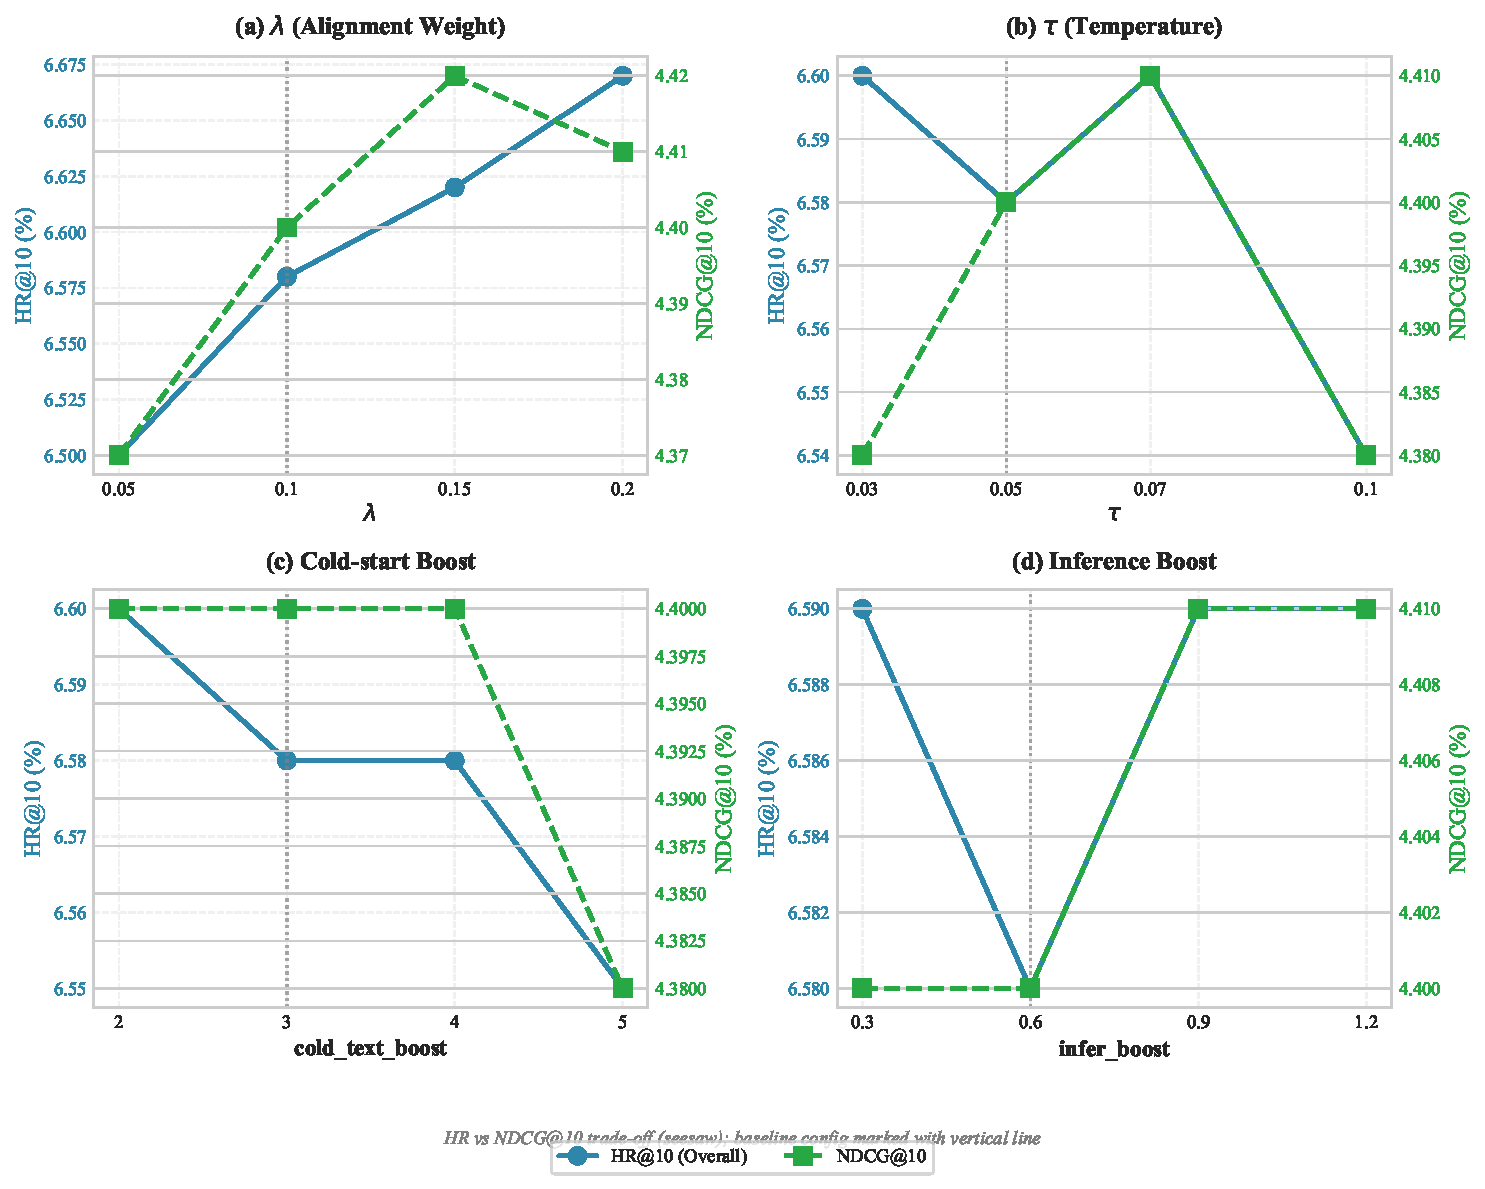
\includegraphics[width=\linewidth]{figures/sensitivity_tradeoff_ndcg.pdf}%
}{%
  \fbox{\parbox[c][0.25\textheight][c]{0.9\linewidth}{\centering
  \textbf{Sensitivity Analysis}\\
  Run \texttt{plot\_sensitivity.py}}}%
}
\caption{Hyperparameter sensitivity on Toys\&Games (7B). Each panel
varies one parameter while holding the others at default values
(dashed vertical line). HR@10 (solid, left axis) and NDCG@10
(dashed, right axis) remain stable across these settings, with
total variation under 0.2 pp for HR@10 and under 0.05 pp for
NDCG@10.}
\label{fig:sensitivity}
\end{figure}

Figure~\ref{fig:sensitivity} shows the sensitivity of \model to
$\lambda$, $\tau$, $\beta$ (Eq.~\eqref{eq:cold_reweight}), and
$\beta_{\text{infer}}$ (Eq.~\eqref{eq:infer_boost}) on Toys\&Games (7B),
plotting HR@10 (left axis) and NDCG@10 (right axis) as each varies
while the others are held at their default values ($\lambda{=}0.10$,
$\tau{=}0.05$, $\beta{=}3.0$, $\beta_{\text{infer}}{=}0.6$).

\paragraph{Alignment weight $\lambda$ and temperature $\tau$.}
Both contrastive hyperparameters show smooth, unimodal curves.
HR@10 ranges from 6.50\% ($\lambda{=}0.05$) to 6.67\%
($\lambda{=}0.20$), a spread of only 0.17 pp; NDCG@10 peaks at
$\lambda{=}0.15$ (4.42\%) and remains within 0.05 pp across the
grid. Temperature $\tau$ is similarly stable: HR@10 varies by
0.06 pp and NDCG@10 by 0.03 pp over the tested range
($0.03$--$0.10$). This confirms that the contrastive objective is
robust to moderate tuning.

\paragraph{Cold-start boost and inference boost.}
The training coefficient $\beta$ (Eq.~\eqref{eq:cold_reweight}) has minimal impact on overall
metrics (HR@10 within 0.05 pp, NDCG@10 within 0.02 pp), as it
primarily affects the training-time reweighting of low-popularity
items. The inference coefficient $\beta_{\text{infer}}$ is similarly stable for overall
performance (HR@10 within 0.01 pp). Consistent with
Eq.~\eqref{eq:infer_boost}, it modulates text reliance for
low-popularity items at inference time; overall HR@10 and
NDCG@10 remain within the narrow bands above across the tested grid.

\paragraph{Takeaway.}
These hyperparameters exhibit low sensitivity on overall metrics,
with total variation under 0.2 pp for HR@10 and under 0.05 pp for
NDCG@10. This makes \model easy to tune in practice: the default
configuration performs near-optimally, and practitioners can adjust
$\lambda$ or $\beta_{\text{infer}}$ to trade off between overall and
cold-start performance without risking large regressions.

\section{Conclusion}
We presented \model, a method that brings explicit cross networks and
multi-view \llm text alignment to sequential recommendation.
Full-ranking experiments on Amazon Beauty and Toys\&Games yield three
actionable takeaways:

\textbf{(1) TF-IDF is a surprisingly strong baseline.}
\tfidf alone provides substantial gains over ID-only baselines
(+2.6\%/+6.3\% HR@10 on Beauty/Toys) and should be the
\emph{first} text enhancement before investing in \llm embeddings.

\textbf{(2) Multi-view improves cold-start ranking under equal bandwidth.}
Under equal embedding bandwidth ($4{\times}64$-d vs.\ $1{\times}256$-d),
multi-view \llm prompting yields the best cold-start ranking quality:
\model achieves the highest NDCG\_new@10 and MRR\_new@10 on both
datasets, while narrowing the HR\_new gap to ID-only on Beauty
(1.76\% vs.\ 1.88\%) and exceeding it on Toys
(2.04\% vs.\ 1.92\%).

\textbf{(3) The cross network governs the HR--MRR/NDCG trade-off.}
Enabling cross sharpens ranking quality (MRR/NDCG) at the cost of
recall (HR); disabling it reverses this balance. This maps directly
to deployment scenarios: disable cross for candidate generation,
enable it for final re-ranking.

\smallskip\noindent
All code and configuration files are available at
\texttt{\url{https://anonymous.4open.science/r/recbole-multiview-D83A}}.

\bibliographystyle{unsrt}
\bibliography{refs}

%% ====================================================================
%% APPENDIX REMOVED for RecSys Main Track Long submission (8pp + refs).
%% All auxiliary analyses are provided in the anonymous repository:
%%   https://anonymous.4open.science/r/recbole-multiview-D83A
%%
%% Contents moved to repo:
%%   - Sampled evaluation sanity check (uni100 vs. full ranking)
%%   - Hyperparameter configurations (Balanced / Cold-Tail-optimized presets)
%%   - Sensitivity analysis on 4 key hyperparameters
%%   - Seed stability analysis (4 seeds)
%%   - Extended strata results (few / frequent)
%% ====================================================================

\end{document}


